\chapter{Grammar}

To begin with I would like to say that grammar is the core of every language. Grammar comprises different themes that are united in a system of changing words enough for building sensible syntax constructions. We will look at Novoslovnica grammar from the point of Parts of Speech.

Part of speech (POS) - is a category of words which have similar grammatical properties.

Thus we unite some words into parts of speech when there are a lot of similar grammar properties, such as “number”, “person”, “case”, “tense” etc. In this chapter we will go through different parts of speech and study what differences they have and how we should deal with them. 

POS have two main categories - independent parts of speech and auxiliary parts of speech. Why some of POS are auxiliary or independent? This refers to their semantic values. Independent POS have a full semantic value. Auxiliary have not. What it means: when you say a word of an independent POS you reproduce some meaning that the interlocutor can recognize.
Example:
River - this word can be recognized by interlocutor as some concept of water flowing in a restricted area.
Beautiful - this word is recognizable as an attribute of any concept that is nice, pleasant to the person (i.e. speaker or interlocutor)
Came - this word can be recognized as any concept’s action of going to the destination point and having reached it. 

And so on. You see that every word has its own meaning, rather full to imagine yourself some information you have been received. This is not true for auxiliary POS. For example, words “and” or “to” cannot give you any map in your mind into any sensible meanings. Though these words have no determined sense itselves, they are extremely important in the whole phrase. English language is an analytical one, that’s why words are mostly connected with each other in the phrase by auxiliary POS. Without them you cannot understand, what the person have said to you. Slavic languages are fusional, but there are enough analytic features in them, hence auxiliary POS are also important.

Also there are two additional categories - particles and interjections. Some allocate them into separate categories, some claim they belong to an auxiliary category. Nevertheless, these are separated POS that have different properties.

Particles add to words they are close to some additional functions. If you delete them from your phrase, there will be no change in the whole meaning (that’s why I cannot say they are an auxiliary ones), but with presence of particles you will get more semantic or emotional information. English language has very few particles. The most known is “to” as an infinitive indicator particle of a verb. Controversially, Slavic languages have a bit more particles, that are rather popular in the spoken language. 
Examples:
Ja sům govoril tobě. - I have told you.
Ja sům govoril že tobě! - I have told you! (Additional semantic meaning. The speaker shifts emphasis from undefined to the word “govoril” (told). So the interlocutor now have a determined emphasis of the phrase. The speaker wants to say that he has already told the same fact to the interlocutor and his idea has become true just now.) 

Interjection is a POS that have no semantic meanings. They are not words in over common comprehension. Interjections are sounds that we produce. It is rather difficult to say sometimes what differences are between interjections and senseless sounds that we can produce (i.e. some spontaneous exclaims, murmuring etc.) Interjections are divided into intended exclaims (with bright emotional color) and sound imitations (i.e. animal voices imitation).

These are categories of POS. If we speak about independent POS, we should take into account that there are different semantic, morphological and syntax functions can be described by these POS. There several type of these functions: the concept, the attribute, the predicate and the demonstrative.

The concept is something that correlates with the object or subject in the real world. It could be either abstract or imaginary, but we can ask a questions “Who? What?” about it.

The predicate is something that determines the action, corresponding to a concept. We often ask questions “What to do?” to reveal a predicate.

The attribute is something that is correspond to a concept or an action. We ask questions “What concept is like?” or “What action is like?” to find out the determine value of the attribute.

The demonstrative points out the concept. It has the same question with the attribute, yet has no semantic value but demonstrating a concept it corresponds with. 

POS with concept properties are Nouns and Cardinal Numerals. POS with attribute properties are Adjectives. Ordinal Numerals and Adverbs. POS with action properties are Verbs, Participles, Gerund. POS with demonstrative attributes are Pronouns.

Thus Noun, Adjective, Verb, Adverb, Numeral, Pronoun, Gerund, Participle are independent while Preposition, Particle, Interjection, Conjunction are auxiliary.

The last division of independent POS is nominal/verbal. It is extremely important, because this division shows differences in grammar of nominal and verbal POS. Verb, Participle, Gerund are verbal POS while Noun, Adjective, Numeral are nominal. Adverbs and pronouns stay separately - the first one because of its immutability and the second one because of its heterogeneity. 

In this chapter we will speak about every POS I have listed above. In the beginning of each paragraph I will give you a table of some kind of property description of the POS.

First you should know some facts about different grammatical properties in Novoslovnica.


\newcounter{casechapter}[section]
\section{Case}

Case\index{case} is a grammatical property of a nominal POS (Part of speech) that shows what references this nominal POS has with other words in a sentence (phrase). This property is widely known in fusional languages, while analytical languages do not often possess this property. Thus, English has only two active cases - Nominative and Oblique one. Moreover, oblique case is used practically only within pronouns while nouns have no such a case. That means case is not the only way to show references between nominal POS and other words in a sentence. Case is just one of the ways to show it and Slavic languages as being fusional widely use this grammar category.

Different Slavic languages have different number of cases. For example, Russian language has six cases while Serbian language has seven. We can find exceptions in Bulgarian and Macedonian languages, which are analytical that is why they have only one case for a noun and adjective and three cases for a pronoun.

Different cases are referred to different semantic links between words. It is the cause why we see ambiguity of cases in different languages (that have different amount of cases and different usage rules of cases). Novoslovnica provides most common and wide means to use cases with almost full determination. When you speak Novoslovnica you have to use the case of exact semantic value and not of the longstanding phraseology of your own language.

With this principle Novoslovnica establishes nine cases. Nine changing patterns that determine alterations of all words of nominal POS. This is the unification of Slavic languages in the sphrere of fusial word linking. Here they are:

\newglossaryentry{nominative}{name=P.C., description={Nominative}}
\newglossaryentry{genitive}{name=G.C., description={Genitive}}
\newglossaryentry{partitive}{name=P.C., description={Partitive}}
\newglossaryentry{accusative}{name=A.C., description={Accusative}}
\newglossaryentry{dative}{name=D.C., description={Dative}}
\newglossaryentry{instrumental}{name=I.C., description={Instrumental}}
\newglossaryentry{prepositional}{name=Pr.C., description={Prepositional}}
\newglossaryentry{locative}{name=L.C., description={Locative}}
\newglossaryentry{vocative}{name=V.C., description={Vocative}}

\begin{itemize}
	\item Nominative (\gls{nominative})
	\item Genitive (\gls{genitive})
	\item Partitive (\gls{partitive})
	\item Dative (\gls{dative})
	\item Accusative (\gls{accusative})
	\item Instrumental (\gls{instrumental})
	\item Prepositional (\gls{prepositional})
	\item Locative (\gls{locative})
	\item Vocative (\gls{vocative})
\end{itemize}

In this chapter we will speak about cases in general. All examples will disclose case features through nouns as examples.

Nominative\index{case!nominative} case (\textit{Imenóvnik}) is used when we are talking about a concept as an actor. If the sentence is full, the subject is in Nominative. You can ask questions like «Who? What?» to it.

This case is basic in most languages, so POSes in this case are supposed to be in the normal form (that we can find in a dictionary). In Novoslovnica nominative also determines a normal from of the word. In the examples you can see full sentenses, where subject is used in nominative.

\textbf{Examples:}

\stepcounter{casechapter}
\arabic{chapter}.\arabic{section}.\arabic{casechapter} \textit{\textbf{Dom}-òt je vëlïkym.} - The \textbf{house} is big.

\stepcounter{casechapter}
\arabic{chapter}.\arabic{section}.\arabic{casechapter} \textit{\textbf{Izučilišto}, de ja sę učam, je starym}. - The \textbf{school} I attend is old.

\stepcounter{casechapter}
\arabic{chapter}.\arabic{section}.\arabic{casechapter} \textit{Klüč-òt je od ovoŭ vråtoŭ.} - The key is to these doors.

Genitive\index{case!genitive} case (\textit{Čyǐnik}) is used when we are talking to an object being related to another one. Thus this case show what generation the object is of and what is it made from or whom does it belong to. The questions that determine the case are «Whose? Which? What?».

In Novoslovnica possessive case equals to genitive one, so English «'s» constructions should be translated in genitive (example 4.1.4). Further, genitive in Novoslovnica could be related to usage of nouns with «of» preposition (example 2, 3).

\textbf{Examples:}

\stepcounter{casechapter}
\arabic{chapter}.\arabic{section}.\arabic{casechapter} \textit{Kniga \textbf{brata} je vëlïmi zajimliva.} — My \textbf{brother}'s book is very fascinating.

\stepcounter{casechapter}
\arabic{chapter}.\arabic{section}.\arabic{casechapter} \textit{Cěna \textbf{uspěha} je mnogo vëlïka.} — The price of \textbf{success} is very high.

\stepcounter{casechapter}
\arabic{chapter}.\arabic{section}.\arabic{casechapter} \textit{Sklad je na koncu \textbf{ulicy}-ta.} — The shop is at the end of the \textbf{street}.

Partitive\index{case!partitive} case (\textit{Ličóvnik}) is used when we are talking about some amount of object having or being supposed to have uncountable properties. The questions that determine the case are «Of what? With what? How much of?».

This case has many coinciding forms with genitive, though in masculine gender it has another endings (examples 1, 3). In English it should be translated with «of» construction (example 1). If uncountable nouns are used with the predicate directly or with adverbs of measure, they should be translated into Oblique case in English (example 2, 3).

\textbf{Examples:}

\stepcounter{casechapter}
\arabic{chapter}.\arabic{section}.\arabic{casechapter} \textit{Daǐ mi čašku \textbf{čaju}.} — Give me a cup of \textbf{tea}.

\stepcounter{casechapter}
\arabic{chapter}.\arabic{section}.\arabic{casechapter} \textit{Dodaǐ do pïroga němnogo \textbf{vody}.} — Add some \textbf{water} to a cake.

\stepcounter{casechapter}
\arabic{chapter}.\arabic{section}.\arabic{casechapter} \textit{Predaǐ mi \textbf{cukru}.} — Pass me \textbf{sugar}.

Dative case (\textit{Datelnik}) is used when we are talking about a noun to which something is given. We can ask a question for a word in this case as «Whom? For whom?».

It's simple with pronouns, because there is a dative case within pronouns in English (example 1). In some use cases we can find a noun with «for» preposition to be translated into Novoslovnica's dative (example 2). However, in these cases form with «dlä» preposition with genitive can be used instead (example 3).

However, there are cases when some direct objects in English will be translated with dative in Novoslovnica (example 4), so you need to consider the semantic value of dative — give somebody something.

\textbf{Examples:}

\stepcounter{casechapter}
\arabic{chapter}.\arabic{section}.\arabic{casechapter} \textit{Kaži \textbf{mi}, čto ty hteš da dostęžiš ovym.} — Tell \textbf{me} what do you want to achieve with this.

\stepcounter{casechapter}
\arabic{chapter}.\arabic{section}.\arabic{casechapter} \textit{Jesòm stvoril podarek \textbf{tatě}.} — I've made a present for \textbf{daddy}.

\stepcounter{casechapter}
\arabic{chapter}.\arabic{section}.\arabic{casechapter} \textit{Jesóm stvoril podarek \textbf{dlä taty}.} — I've made a present \textbf{for daddy}.

\stepcounter{casechapter}
\arabic{chapter}.\arabic{section}.\arabic{casechapter} \textit{Jesòm podal \textbf{bratu} moju pomočj, dy on zapytaše mę o tom.} — I helped my \textbf{brother}, when he asked about it.

Accusative\index{case!accusative} case (\textit{Vinitelnik}) is used to describe a direct object of the action. The questions determining the case are «What? Whom?».

If a noun has a role of a direct object in English sentense (Oblique case), you should translate it with accusative in Novoslovnica (example 1-3).

\textbf{Examples:}

\stepcounter{casechapter}
\arabic{chapter}.\arabic{section}.\arabic{casechapter} \textit{Ja viđu lěpyǐ \textbf{lěs} predò mnom.} — I see a beautiful \textbf{forest} ahead of me.

\stepcounter{casechapter}
\arabic{chapter}.\arabic{section}.\arabic{casechapter} \textit{On pokazaše mi \textbf{kota}, ke glåsisto kričěše.} — He showed me a \textbf{cat}, crying loudly.

\stepcounter{casechapter}
\arabic{chapter}.\arabic{section}.\arabic{casechapter} \textit{Znaš li ty \textbf{rěku}, če tëče z severu na jug?} — Do you know a \textbf{river} that flows from north to south?

Instrumental\index{case!instrumental} case (\textit{Tvornik}) is used to describe an instrument of an action that affects the object of the action. The questions related with this case are: «With whom? With what?».

As you can see from auxiliary questions, English phrases with «with» expressions should be translated to instrumental case in Novoslovnica. Moreover, «by» expressions also are translated to instrumental case. The difference is in preposition:

\begin{table}
	\begin{tabular}{p{9em}p{9em}}
		«with»-expressions are translated in & «s»+instrumental case (keeping preposition) with animate nouns or pronouns (examples 17, 18)
		instrumental case (loosing preposition) with inanimate nouns (example 20) \\
		«by»-expressions are translated in &  instrumental case, loosing preposition (example 19) \\
	\end{tabular}
\end{table}

\textbf{Examples:}

\stepcounter{casechapter}
\arabic{chapter}.\arabic{section}.\arabic{casechapter}\textit{Idaǐ na věčôrku sò \textbf{mnom}.} — Let's go to the party with \textbf{me}.

\stepcounter{casechapter}
\arabic{chapter}.\arabic{section}.\arabic{casechapter} \textit{Kaži mi, s \textbf{kym} ty hteš poǐdati na věčôrku?} — Tell me, with \textbf{whom} do you want to go to the party?

\stepcounter{casechapter}
\arabic{chapter}.\arabic{section}.\arabic{casechapter} \textit{Kniga-ta je napisana vëlïkym \textbf{tvorcom}.} — The book is written by a great \textbf{author}.

\stepcounter{casechapter}
\arabic{chapter}.\arabic{section}.\arabic{casechapter} \textit{Ta búda je vybúdana \textbf{kamenom}.} — That building is built with \textbf{stone}.

Prepositional\index{case!prepositional} case (\textit{Predložnik}) is used when something is an object of speaking. It can be related to auxiliary questions «About what? About whom?».

In English there are two prepositions that show that it should be translated to prepositional case in Novoslovnica — «about», «of». Note, that you should divide phrases with the object of speaking from phrases with genitive forms.

This case is called prepositional in Novoslovnica, because it is used only with preposition «o» (about).

\textbf{Examples:}

\stepcounter{casechapter}
\arabic{chapter}.\arabic{section}.\arabic{casechapter} \textit{Råzkaži mi o tom \textbf{slučajě}.} — Tell me about that \textbf{case}.

\stepcounter{casechapter}
\arabic{chapter}.\arabic{section}.\arabic{casechapter} \textit{On ne zna ničto o tom \textbf{městě}.} — He knows nothing about that \textbf{place}.

\stepcounter{casechapter}
\arabic{chapter}.\arabic{section}.\arabic{casechapter} \textit{Ja ne kazal sòm mu ničto o \textbf{sobě}.} — I have told nothing to him about \textbf{myself}.

Locative\index{case!locative} case (\textit{Městnik}) is used when we speak about something as a place where the action related with the predicate takes place. It can be related to an auxiliary question: «where?».

In English phrases with both «at» and «in» prepositions should be translated to locative in Novoslovnica (examples 1-3). Note, that «in» preposition is usually translated with locative, while «into» preposition should be translated with accusative (example 4).

\textbf{Examples:}

\stepcounter{casechapter}
\arabic{chapter}.\arabic{section}.\arabic{casechapter} \textit{Hođu v \textbf{lěsu}.} — I am walking in the \textbf{forest}.

\stepcounter{casechapter}
\arabic{chapter}.\arabic{section}.\arabic{casechapter} \textit{Ja běše v \textbf{domu}, koĝda ty pozovaše mę izvòn.} — I was at \textbf{home}, when you called me out.

\stepcounter{casechapter}
\arabic{chapter}.\arabic{section}.\arabic{casechapter} \textit{On živa v golěmomu \textbf{grådu}.} — He lives in a big \textbf{city}.

\stepcounter{casechapter}
\arabic{chapter}.\arabic{section}.\arabic{casechapter} \textit{Hođu v \textbf{lěs}.} — I am walking into the \textbf{forest}.

Vocative\index{case!vocative} case (\textit{Zvatelnik}) is a special case in Novoslovnica that binds a new object to the action by direct mentioning it.

Vocative is usually used with human names (example 28) or animate nouns (example 29), but can also be used with every noun that is supposed to be a receiver of an action result (example 30).

Vocative is usually divided from the main sentense by a comma.

\textbf{Examples:}

\stepcounter{casechapter}
\arabic{chapter}.\arabic{section}.\arabic{casechapter} \textit{\textbf{Ivane}, začto ne odgovořaš mi?} — \textbf{Ivan}, why don't you answer me?

\stepcounter{casechapter}
\arabic{chapter}.\arabic{section}.\arabic{casechapter} \textit{\textbf{Otče}, koĝda hte mi kupiš dvojokol?} — \textbf{Father}, when will you buy me a bike?

\stepcounter{casechapter}
\arabic{chapter}.\arabic{section}.\arabic{casechapter} \textit{\textbf{Větre}, začto ne sę zaspokojiš?} — The \textbf{Wind}, why don't you calm down?

These cases cover 99,99\% of possible nominal POS declension. Some extra ordinary cases exist, but they should not be mentioned here.

\section{Number}

How do people understand what is the numeric characteristic of the object? Of course, the simple way is to use numerals. We can call to a numeral and link it with some noun, thus, people will understand that there is an amount shown by a numeral of the concept shown by a noun. But it is rather uncomfortable to use near every noun an additional numeral. That’s why there is a concept of a number.

Number shows what is the amount of some concept without using numeral before the noun.

Number is a grammar property of the word, its alteration. That means when we change number of the word, we change the word itself and not add some additional words or particles around the word we are speaking about.

There are three numbers in Novoslovnica: Singular, Dual and Plural. Singular and Plural are familiar to an English speaker. Dual is rather peculiar, so I should take additional account on it.

Dual number is used when we speak about a pair of something - hands, legs, eyes etc. of one person. Two-doors gates, two boolean values, two antipodes etc. In these cases we use a dual number. Dual depends on the word which is spoken, that is why we cannot determine a static rule about choosing a form for a dual number. We can get a dual form of the word by using a declension function with a type of declension corresponding with the word.

The last form we should speak about is a counting form. Counting form is used with the nouns. It occurs when we use the noun with the numerals “Two”, “Three” or “Four” (cardinal numbers). The counting form is equal to a dual number in writing. 

\textbf{Examples:}

\textit{Dva doma} (two houses) - counting form

\textit{Doma} (two ones) - dual number

\textit{Tri doma} (three houses) - counting form

\textit{Domy} (three ones) - plural number 

\section{Person}

This grammar category\index{person} determines the person who is spoken about. There are three points of view:

\begin{itemize}
	\item the point of the speaker (First person)
	\item the point of the interlocutor (Second person)
	\item the point of other persons, that are not involved into discussion (Third person)
\end{itemize}

That is how a Slavic discussion could be seen. Practically, this concept is similar to all European languages, particularly English. There is a total equivalency with English in Novoslovnica, so it is not necessary to describe the usage all of these person types. Just look at the following examples to get sure of it:

\textbf{Examples:}

\textit{Ja glědaju v prozorec cěl věčôr.} - I am looking outside the window for the whole evening. (The first person)

\textit{Vy kažete že sámo ïsto byše včera? }- Do you mean that the very same thing was yesterday? (The second person)

\textit{Ony hlåpcy niĝda ne mogut pjiti tïho.} - Those guys never can drink quitely. (The third person)

\section{Tense}

Grammatical tense\index{tense} is a category that expresses time reference with reference to the moment of speaking. In many languages there are three main categories of present, past and future, that refer to the moment of speaking, the period before and the period after it respectively. English belongs to the group of languages with tense-rich grammar. It has 16 tenses, divided by categories of time and perfection. Novoslovnica has 12 tenses, based on the two principles like English. They are:

\begin{itemize}
	\item Present Indefinite Tense
	\item Present Definite Tense
	\item Future Indefinite Tense
	\item Future Definite Tense
	\item Pre-future Tense
	\item Future-in-the-Past Tense
	\item Pre-future-in-the-Past Tense
	\item Aorist
	\item Perfect
	\item Imperfect
	\item Plusquamperfect
	\item Past Indefinite Tense
\end{itemize}

First two tenses describe the present moment, the next three ones refer to the future period of time and the last six ones describe the period of time that has already passed.

We can divide past tenses in two groups - past tenses itself and future-in-the-past tenses, that describe actions that refer to the future moment with reference to the moment in the past.

Novoslovnica tense system can be described better with the help of the following diagram:

\begin{figure}
	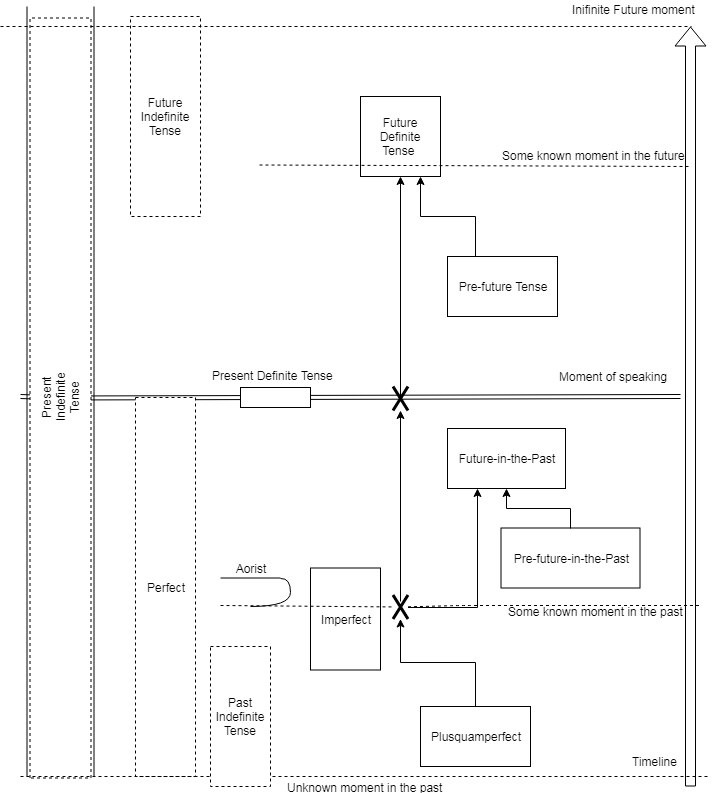
\includegraphics[width=\linewidth]{./sources/tenses.jpg}
	\caption{Tenses in Novoslovnica}
	\label{fig:tenses}
\end{figure}

Present group of tenses consists of Present Indefinite Tense (\textit{Pritomen čas}) and Present Definite Tense (\textit{Sëdyšen čas}).

Present Indefinite Tense\index{tense!present indefinite} (\textit{Pritomen čas}) is used when the action does not depend on time. For example, in the first example we know that the Earth always revolves and nothing but the apocalypsis can change it. This tense is very similar to the English one and has similar use cases. We can find this tense in indicative (examples 1, 2) and declarative (example 3, 4) moods mostly (in some cases it can be found in different moods too).

Note that in declarative there are two variants of present indefinite, because of its resultive semantics. In example 3 you can see the verb in declarative mood, in present indefinite tense, and in example 4 you can see the same tense and mood but within a predicateless sentence.

Also take care of the translation in example 3. You can mess it with English Present Perfect Tense (He has bought two cars), but this sentence should be translated with the verb «to have» in Present Indefinite with the participle III of the verb «to buy» (bought).

\textbf{Examples:}

\textit{Zemlä sę vreta okolo slånca.} - The Earth revolves around the Sun.

\textit{Vsękyǐ denj ja hođam do učilišta prez lěpyǐ park.} — Every day I walk to school through the beautiful park.

\textit{On imá kupeno dva vozidla.} — He has two cars bought.

\textit{Lěs i tïhota...} — There are forest and silence around me...

Present Definite Tense\index{tense!present definite} (\textit{Sëdyšen čas}) is used if the action depends on time. In the first example we can see a sentense with the following semantics: now I think about the rest, though in an hour I can forget about this thought.

Generally, this tense is close to Present Continuous Tense in English, though has a different interpretation. If you want to get in differences, we can give you such an example: «The Earth is revolving around the Sun at the moment». Read this hypothetic sentence that is syntaxicly valid in English.

What would be the differences of English and Novoslovnica here? It is in a term of differentiation. English operates with the time and Novoslovnica operates with the mutability. That is why here Novoslovnica will still use Present Indefinite Tense with the word «sëdy» (at the moment).

\textbf{Examples:}

\textit{Ja myslü o počïvkě.} — I am thinking about the rest.

\textit{On idaje do råboty, zato ne može da odgovori vam.} — He is going to the work, that is why he cannot answer you.

The group of future tenses comprises two ones: Future Tense and Pre-future Tense.

Future Definite Tense\index{tense!future definite} (\textit{Bųdešt čas}) defines that the action will appear in the future with reference with the moment of speaking. There are three variants of how you can use Future Tense in Novoslovnica.

Firstly, you can use the verb «hteti» (to will) in 3-person form with the main verb in Present Indefinite Tense (example 1). This varitant is most similar to English Future Simple Tense.

Secondly, you can use the verb «byti» (to be) with inifinitive form of the main verb (example 2). This variant is close to English Future Continuous Tense. It is often used with verbs of A-type (read the chapter about verbal types in Novoslovnica).

Finally, you can use a synthetic verb form with the future tense conjugation (example 3). In English, it should be translated in Future Simple so as the first one.

\textbf{Examples:}

\textit{Ja hte kazam ti něčto.} — I will tell you something.

\textit{Ja bųdu sluhati gudbu.} — I will listen to music. (I will be listening to music).

\textit{Nakonec ja tę viđahtem}. – Finally, I will meet you.

Pre-future Tense\index{tense!pre-future} (\textit{Predbųdešt čas}) is a grammatical tense that is used when the speaker should explicitly show that the action will take place before another future action. So, this tense deals with the comparison of future actions rather than with the moment of speaking.

In Novoslovnica Pre-future Tense is formed by using the verb «hteti» in 3-person form with the main verb in perfect form (examples 1, 2). This tense should be translated in English with Future Perfect Tense.

\textbf{Examples:}

\textit{Ja hte sòm kupil květy, dy ty hte priǐdaš do města.} — I will have bought flowers, when you come to the place.

\textit{On hte je zakončil učilišto, dy otec mu hte sę vreta dodomu}. — He will have graduated from school, when his father comes back home.

Future Indefinite Tense\index{tense!future indefinite} (\textit{Něĝdašen čas}) is a rather rare tense to be used in Novoslovnica. It has no direct equivalents in English and should be translated in Future Simple with some keywords (such as «somewhen», «ever», «once»). The sense of this tense is to show that the action takes place in a future moment or period of time, but we do not care of when it will occur or how long it will last.
This tense is formed by Pre-future form of the verb «byti» with the past passive participle of the main verb. Look at the examples to get acquainted.

\textbf{Examples:}

\textit{On hte je byl nagrådil medalom mę.} — Once he will grant me with a medal.

\textit{Ja hte sòm byl kupil vašu věčj.} — Once I will but your item.

All other tenses are related to the past period of time. Firstly, we will consider real past tenses and then future-in-the-past ones.

Aorist\index{tense!aorist} (\textit{Prost minul čas}) determines the fact of the committed action without semantic details. It is similar in usage with English Past Simple Tense. Using Aorist we consider only the time the action occurs, but do not think about its duration.

In Novoslovnica it is formed by verb-base vowels with past definite endings: «-h», «-ša», «-še», «-hma», «-hta», «-ha», «-hme», «-hte», «-hu».

\textbf{Examples:}

\textit{Ja dělah råbotu-ta včera.} — I did the work yesterday.

\textit{Pred dvě ročiny ja jěŝih v gråd-òt.} — Two years ago I travelled to the city.

Imperfect\index{tense!imperfect} (\textit{Neporęden minul čas}) determines the imperfect aspect of the past action. That means it is used with habitual, durable repeated actions etc, that took place in the past. Using imperfect we add the information, that our action took some exact time in the past. This tense is similar in usage with English Past Continuous Tense or Past Perfect.

It is formed so as Aorist with the one difference. There is a «-ě-» vowel before endings, not the verb-base vowel. So, for any verb type (see a chapter about verbal types) there is only a single imperfect form.

\textbf{Examples:}

\textit{Ja pišěh nadomnu råbotu dvě godiny včera.} — I was writing my homework for two hours yesterday.

\textit{Prijatelj mi ráděše na zavodu dvě ročiny.} — My friend had worked on a plant for two years.

Perfect\index{tense!prefect} (\textit{Svòršen minul čas}) determines the action has been committed before the present moment. That means, that we take account on the result of the action, on the fact it is finished, while Aorist determines the fact of the action itself and the time when it occured. So, it is a full equivalent of English Present Perfect Tense.

In Novoslovnica Perfect is formed by the auxiliary verb «byti» in Present Indefinite and an L-participle following it.

\textbf{Examples:}

\textit{On je izmyslïl novu ŧeoriju o problemě-ta.} — He has devised a new theory on the problem.

\textit{Môǐ brat je zakončil vysšojučilišto.} — My brother has graduated from University.

Plusquamperfect\index{tense!plusquamperfect} (\textit{Predminul čas}) determines the fact our action is further from us than another action in the past. It is akin Pre-Future tense, just with past actions. Simply speaking, it is an equivalent of English Past Perfect Tense. So as Pre-Future tense, actions in Plusquamperfect are usually used in pair with another past action that stands in Aorist.

Plusquamperfect in Novoslovnica is formed with aorist form of the auxiliary verb «byti» with an L-participle of the main verb.

\textbf{Examples:}

\textit{Ja byh doǐdal do ulicy-ta, dy on mi odŝvoniše, če ne može da priǐde.} — I had arrived to the street by the time he called be to say he cannot come.

\textit{On byše zdělal model, ĝda ja kazaše mu, če to ne máše potrěbnostï.} — He had done a model, when I told him it was unnecessary. 

Now we should consider two last tenses: Future-in-the-Past tense and Pre-Future-in-the-Past tense.

Future-in-the-Past tense (Bųdešt v minulom čas) is used when we speak about past actions, that occured after some other past actions. To emphasize this fact we use a past variant of the future tense — Future-in-the-Past. English has an equivalent, so it is easy to build a parallel between these two tenses. In Novoslovnica this tense is build with imperfect of the auxiliary verb «hteti» and DA-construction of the main verb (example 1).

This tense has also another meaning, that can be expressed with «would like to» phrase in English. It shows a polite intention to do something (example 2).

\textbf{Examples:}

\textit{My zapytahme dali vozidlo htěše da priǐde včas.} — We wondered if the bus would arrive on time.

\textit{Ja htěh da kazam ti něčto.} — I would like to say you something.

Pre-Future-in-the-Past Tense\index{tense!pre-future-in-the-past} (\textit{Predbųdešt v minulom čas}) is used, when we speak about some actions, that happened earlier than some future actions in the past (analogue of pre-future tense in the past). It has a similar meaning with Future-in-the-Past Perfect tense in English and it is rather rarely used.

It is formed with imperfect of the auxiliary verb «hteti» with perfect form of the main verb via DA-construction (look at the example).

\textbf{Examples:}

\textit{Vy kazahte, če htěhte da jeste podpisali pismo pred tym, kak htěhte da započïnate råbotati.} — You said you would have signed the paper before you would start working.

Past Indefinite Tense\index{tense!past indefinite} (\textit{Davnominul čas}) is the last official tense in Novoslovnica. It describes an action that occured in some moment in the past we do not know. In English we should translate it with Past Simple or with the «used to»-construction. It can be considered as a pair to Future Indefinite Tense.

\textbf{Examples:}

\textit{On je byl pisal knigu.} — He used to write a book.

Let us summarize all the equivalents of Novoslovnica's Tenses in English in the next table.

\begin{table}
	\caption{English equivalents of tenses in Novoslovnica}
	\begin{tabular}{ p{11em} p{11em} }
		\textbf{Tense in Novoslovnica}       & \textbf{English equivalent}                  \\
		Present Indefinite Tense             & Present Simple                               \\
		Present Definite Tense               & Present Continuous                           \\
		Future Indefinite Tense              & “once” + Future Simple                       \\
		Future Definite Tense (with “hteti”) & Future Simple                                \\
		Future Definite Tense (with “byti”)  & Future Continuous                            \\
		Future Definite Tense (single form)  & Future Simple                                \\
		Pre-future Tense                     & Future Perfect (Cont.)                       \\
		Future-in-the-Past Tense             & Future-in-the-Past Simple or “would like to” \\
		Pre-future-in-the-Past Tense         & Future-in-the-Past Perfect (Cont.)           \\
		Aorist                               & Past Simple                                  \\
		Perfect                              & Present Perfect (Cont.)                      \\
		Imperfect                            & Past Continuous                              \\
		Plusquamperfect                      & Past Perfect (Cont.)                         \\
		Past Indefinite Tense                & “used to”                                    
	\end{tabular}
\end{table}

The third verbal category can be found in Novoslovnica which is shown only in differences between Aorist and Imperfect: perfection, while other tenses differ only by determinacy and time. So, you can use complex tenses as Perfect, Plusquamperfect, Past Indefinite etc. with aorist and imperfect participles and receive two shades of perfection meaning.

\section{Mood}

% TODO: Check the correspondence with the article

Mood is a grammatical feature of verbs, used for signaling modality []. Mood is distinct from grammatical tense or grammatical aspect, although the same word patterns are used for expressing more than one of these meanings at the same time. There are several moods in Novoslovnica \cite{nsl-naklony}:

\begin{itemize}
	\item Indicative
	\item Declarative
	\item Subjunctive
	\item Conjunctive I
	\item Conjunctive II
	\item Imperative
	\item Optative
	\item Jussive
	\item Hortative
	\item Supine
	\item Inferential
\end{itemize}

Moods are divided into realis and irrealis moods. Realis mood is a grammatical mood which is used principally to indicate that something is a statement of fact. More precisely, it is used to express what the speaker considers to be a known state of affairs. Novoslovnica has two realis moods - indicative and declarative.

Indicative mood (\textit{Oznamitelnyǐ})  is used when we need simply to indicate that something is a statement of fact. Indicative has a variety of forms, including positive, negative and interrogative. Due to this fact it is chosen to be a basic mood, that is compared to the others. Indicative mood will be extensively considered in the next chapters. Just look at few examples.

\textbf{Examples:}

\textit{On glěděše iz prozorca doma si.} - He was looking out of the window of his house.

\textit{Ja bųdu hoditi vò vysšojučilišto črez dvě godiny.} - I will attend the university in two years.

Declarative mood (\textit{Objavitelnyǐ}) is used when we describe a state of something, considering the action it was caused by. Declarative mood is of the same degree of variety as indicative mood, though is not used as often as indicative.

The first difference with indicative mood is in using auxiliary verb “imáti” (to have) instead of “byti” (to be) while forming sentences. This makes some semantic shifts in Novoslovnica. Look at the second example: the auxiliary verb is used in present tense, though it has a resultive semantic value. For present semantics the verbless sentences are used (first example).

The second difference is in the particle being used with the auxiliary verb in two moods. In indicative we use L-particles, while in declarative mood we use passive ones.

\textbf{Examples:}

\textit{Rěka krasna i slånco.} - (There are) Beautiful river and the sun (around me).

\textit{Ja mám rođeno dvôh synoŭ.} - I have two sons born.

Subjunctive mood (\textit{Predpokladnyǐ}) is used when we want to express various states of unreality: wish, emotion, possibility, obligation etc. Subjunctives occur most often, although not exclusively, in subordinate clauses, using particles “aby”, “žeby”, “čtoby”, “išby” (example 1).

Take a note about absence of auxiliary verb while using L-particles. We just use a subjunctive particle with them. Though, we can also use infinitive instead of L-particle with the object in dative (example 2). Moreover, DA-forms can be used to express subjunctive (example 3). Nevertheless, there are cases you can use subjunctive in the main clause (example 4). 

\textbf{Examples:}

\textit{Az upëram aby ty odidal.} - I would like you to leave.

\textit{Az upëram aby ti odidati.} - It’s better for you to leave.

\textit{Ja htem da ty odidaš.} - I want you to leave.

\textit{Ty by odidal odde.} - You better leave here.

Conjunctive mood I (\textit{Domyselnyǐ}) is used to express real wishes relatively present moment. It means, using conjunctive I we show that our wish is still able to be implemented. It is a classic variant of conjunctive and is formed by conjunctive form of the verb “byti” (to be) with an L-participle.

In fact, this mood is rather similar to Conditional II in English with the same tense analogues used (examples 2, 3). If we use just conjunctive clause, it is similar with “wish-construction” usage area in English (example 1). However, we can express conjunctive with the single clause using past transgressive (example 4).

Note, that having two clauses we need to use conditional conjunctions (“ako”, “jestjli”, “koli”, “dali”, “či” etc.).

\textbf{Examples:}

\textit{Az bih htěl da viđu slånco v ovyǐ obvlåčnyǐ denj.} - I wish I see the sun in this cloudy day.

\textit{On biše doǐdal do nas, ako my zazovahme ĝo.} - He would come if we called him.

\textit{Ako znaše on novoslovnicu, mogal biše da govori so vsïmi slověnami.} - If he knew Novoslovnica, he would speak with all Slavs.

\textit{Znavšy novoslovnicu, on mogal biše da govori so vsïmi slověnami}. - If he knew Novoslovnica, he would speak with all Slavs.

Conjunctive mood II (\textit{Domyselnyǐ}) is the second conjunctive mood and it is used to express unreal wishes that have not been realized relatively a moment in the past. It can be formed by the verb “byti” in conjunctive form either  with supine (example 1) or with plusquamperfekt form of the main verb (example 2). It can be related to Conditional III in English. 

Note, that using supine you do not have to use conditional conjunctions between clauses. Moreover, we can use past active participle in the conditional clause (example 3). Attention! Compare this with the past transgressive in the single clause in Conjunctive I.

\textbf{Examples:}

\textit{Htětj da sę vidim s nim včera, bih byl mogal to da sdělam.} - If  I had wanted to see him yesterday, I would have meet him.

\textit{Ako byh htel da sę vidim s nim včera, bih byl mogal to da sdělam.} - If  I had wanted to see him yesterday, I would have meet him.

\textit{Ako byh htel da sę vidim s nim včera, bih byl mogavšym to sdělati.} - the same translation

Imperative mood (\textit{Zapovědnyǐ})  is used when we want to tell somebody a command or a request. In Novoslovnica it has only I-person (in dual and plural) and II-person (in singular, dual and plural) forms. It is indicated by special endings (look forward for details). In the examples you can see how imperative is used.

Please note that imperative is indicated only by single form. Complex forms are not of this mood.

\textbf{Examples:}

\textit{Piši ovu knigu.} - [Please] write this book. (you, sg)

\textit{Kažite mu poslanije-to.} - [Please] tell him the message. (you, pl)

\textit{Pročitaǐte ovu knigu.} - [Please] read this book. (you, pl)

\textit{Predgotuǐmo juž sëdy pokôǐ-ot.} - [Please] prepare the room now! (we, pl)

Optative mood (\textit{Žadatelnyǐ}) is a grammatical mood that expresses wish or hope. It is used when we want something or somebody to let us succeed in any action we are going to do. It is formed by DA-construction in the main clause (look at the examples). 

In English we can find similarity in LET-forms (examples 1, 2) or some general expressions that reveal our wish (example 3).

\textbf{Examples:}

\textit{Da daǐ mi pomognuti ti.} - Let me help you.

\textit{Da bųde tako.} - Let it be so.

\textit{Da žive Bòlĝarija.} - Long live Bulgaria.

Jussive mood (\textit{Umožnitelnyǐ}) is a grammatical mood of verbs for issuing orders and commanding. In Novoslovnica it is used to make orders for third-person expressions. There are no direct equivalents in English for this mood, but we can translate it with impersonal sentences (example 1) or with MUST-modal expressions. It is formed by indicative with “haǐ” modal word.

\textbf{Examples:}

\textit{Haǐ toǐ ne tòpta trevy.} - Do not walk on grass.

\textit{Haǐ on podide.} - He must come closer.

Hortative mood (\textit{Predložnyǐ})  is a grammatical mood that let verb express encourage or discourage of doing something. It can be translated with “let us” (encourage) or “might not” (discourage) constructions in English. In Novoslovnica it is formed with “něhaǐ” modal word with indicative and is able to have negative (example 4) and positive (examples 1-3) form. It is generally used just with I-person expressions.

\textbf{Examples:}

\textit{Něhaǐ grame v ovu gru.} - Let us play this game.

\textit{Něhaǐ pějama pěsnü.} - Let us (both) sing a song.

\textit{Něhaǐ govorim to otcu.} - I might say this to father.

\textit{Něhaǐ ne idame v dom-òt.} - We might not go into the house.


Supine (\textit{Dostęgatelnyǐ}) is rather a grammar form than a mood. Nevertheless, it is often used to express aiming something and the action of approaching to the goal that has been defined. It is similar to infinitive but the ending (infinitive has “-ti” ending, while supine has “-tj” endind). It is usually used with modal verbs and verbs of moving.

Supine can be translated in English through complex predicate. That is because in Novoslovnica supine is practically never used as a single verb form. It is generally used with main verb that determine the background action of the circumstance. Look at the examples to get acquainted with it.

\textbf{Examples:}

\textit{Moǐca je priǐdala povědatj dobru novinu.} - Mojca has come to message a good news.

\textit{Běgi skoro sę preoblekatj.} - Run fast to change clothes.

\textit{Poǐdame kupovatj.} - Let’s go to buy something.

Inferential mood (\textit{Prekazatelnyǐ}) is used to report an unwitnessed event without confirming it. It is often used in stories or fiction books and is very similar with indicative. The only difference is in 3-person in past tenses, where the auxiliary verb “byti” disappears and we use just L-participle. In English it should be translated with ordinary indicative (examples 1-4), sometimes “there”-forms also can be used (example 5). Not, that we use L-participle in Novoslovnica in the past tense (you can mess it with Perfect tense), while it should be translated in Past Simple.
Look at the examples.

\textbf{Examples:}

\textit{Jesòm mu ĝo kupil.} - I have bought it for him.

\textit{Byl sòm kupil naǐ-prosty martenicy, ale toǐ izbral naǐ-råzkošny.} - I had bought simpliest martenitsy, but he bought the most luxurious.

\textit{On byl bogatym.} - He was rich.

\textit{Kųde byl master?} - Where was the master?

\textit{Žila žena i mųž v malomu domu.} - There lived a woman and a man in a small house.

\section{Noun}

\begin{table}[h]
	\caption{Noun characteristics}
	\begin{tabular}{lllll}
		\textbf{Title}              & \textbf{Value}                            \\
		Semantic value              & Concept                                   \\
		Category                    & Independent                               \\
		Subcategory                 & Nominal                                   \\
		Alteration                  & Declension                                \\
		Alteration parameters       & Case, Numbers, Gender, Type of Declension \\
		Differentiation parameters  & Gender, Animacy, Types of  Declension                                  
	\end{tabular}
\end{table}

Nouns can be differentiated by three parameters: gender, animacy and the type of declension.

\underline{Animacy} determines whether the object is animate (we are able to ask “Who is it?” to the object) and inanimate (we are able to ask “What is it?” to the object).

\underline{Gender} determines whether the object is masculine, feminine or undefined (we cannot say it is one of the previous genders). Hence, there are three genders: masculine (with masculine properties), feminine (with feminine properties) and neutral (with undefined properties).

Despite English, Novoslovnica make us always show word gender explicitly of both animacies. We can say “it” to the object if we aren’t coupled with it in English. In Novoslovnica (as in every Slavic language) we should use the predefined gender when we speak about some concept (noun). Using wrong genders shows your ignorance and language nescience.

\underline{Type of declension} is a parameter of declension function. Declension is a function of word alteration. It has two input parameters - the word itself and the type of declension that includes the terms of animacy, gender and some morphological features (such as word endings) in it. The output is a list of forms that the noun can be changed into. Novoslovnica supports 27-cell output list with (3 numbers) * (9 cases) elements in it. Further you can see tables of different declension types. These tables cover all use cases of declension function.

P.S. In tables abbrevs “A” and “I” are for “animate” and “inanimate” respectively.


\begin{table}
	\caption{Hard feminine}
	\begin{tabular}{lllllll}
		\textbf{Ia Type}       
			& \multicolumn{2}{c}{Singular} 
				& \multicolumn{2}{c}{Dual} 
					& \multicolumn{2}{c}{Plural} \\
		& An.   & Inan.  & An.   & Inan.   & An.  & Inan. \\
		Nominative    & \multicolumn{2}{c}{-a}      
						& \multicolumn{2}{c}{-ě}        
							& \multicolumn{2}{c}{-y} \\
		Genitive      & \multicolumn{2}{c}{-y}       
						& \multicolumn{2}{c}{-oŭ}      
							& \multicolumn{2}{c}{-}   \\
		Partitive     & \multicolumn{2}{c}{-y}       
						& \multicolumn{2}{c}{-oŭ}      
							& \multicolumn{2}{c}{-} \\
		Accusative    & \multicolumn{2}{c}{-u}       
						& -ova & -ě
							& \multicolumn{2}{c}{-} \\
		Dative        & \multicolumn{2}{c}{-ě}       
						& \multicolumn{2}{c}{-oma}     
							& \multicolumn{2}{c}{-am} \\
		Instrumental  & \multicolumn{2}{c}{-oǐ}     
						 & \multicolumn{2}{c}{-ama}     
						 	& \multicolumn{2}{c}{-ami} \\
		Prepositional & \multicolumn{2}{c}{-ě}       
						& \multicolumn{2}{c}{-ověh}     
							& \multicolumn{2}{c}{-ěh} \\
		Locative      & \multicolumn{2}{c}{-jï}      
						& \multicolumn{2}{c}{-oŭ}       
							& \multicolumn{2}{c}{-ah} \\ 
		Vocative      & \multicolumn{2}{c}{-o}       
						& \multicolumn{2}{c}{-ove}      
							& \multicolumn{2}{c}{-ije}
	\end{tabular}
\end{table}


\begin{table}
	\caption{Hard masculine}
	\begin{tabular}{lllllll}
		\textbf{Ib Type}       
		& \multicolumn{2}{c}{Singular} 
		& \multicolumn{2}{c}{Dual} 
		& \multicolumn{2}{c}{Plural} \\
		& An.   & Inan.  & An.   & Inan.   & An.  & Inan. \\
		Nominative    & \multicolumn{2}{c}{-a}      
		& \multicolumn{2}{c}{-ě}        
		& \multicolumn{2}{c}{-y} \\
		Genitive      & \multicolumn{2}{c}{-y}       
		& \multicolumn{2}{c}{-oŭ}      
		& \multicolumn{2}{c}{-}   \\
		Partitive     & \multicolumn{2}{c}{-y}       
		& \multicolumn{2}{c}{-oŭ}      
		& \multicolumn{2}{c}{-} \\
		Accusative    & \multicolumn{2}{c}{-u}       
		& \multicolumn{2}{c}{-ě}
		& \multicolumn{2}{c}{-y} \\
		Dative        & \multicolumn{2}{c}{-ě}       
		& \multicolumn{2}{c}{-oma}     
		& \multicolumn{2}{c}{-am} \\
		Instrumental  & \multicolumn{2}{c}{-oǐ}     
		& \multicolumn{2}{c}{-ama}     
		& \multicolumn{2}{c}{-ami} \\
		Prepositional & \multicolumn{2}{c}{-ě}       
		& \multicolumn{2}{c}{-ověh}     
		& \multicolumn{2}{c}{-ěh} \\
		Locative      & \multicolumn{2}{c}{-jï}      
		& \multicolumn{2}{c}{-oŭ}       
		& \multicolumn{2}{c}{-ah} \\ 
		Vocative      & \multicolumn{2}{c}{-o}       
		& \multicolumn{2}{c}{-ove}      
		& \multicolumn{2}{c}{-ije}
	\end{tabular}
\end{table}

\begin{table}
	\caption{Soft feminine}
	\begin{tabular}{lllllll}
		\textbf{Ic Type}       
		& \multicolumn{2}{c}{Singular} 
		& \multicolumn{2}{c}{Dual} 
		& \multicolumn{2}{c}{Plural} \\
		& An.   & Inan.  & An.   & Inan.   & An.  & Inan. \\
		Nominative    & \multicolumn{2}{c}{-ä}      
		& \multicolumn{2}{c}{-ě}        
		& \multicolumn{2}{c}{-ï} \\
		Genitive      & \multicolumn{2}{c}{-ï}       
		& \multicolumn{2}{c}{-öŭ}      
		& \multicolumn{2}{c}{-ëǐ}   \\
		Partitive     & \multicolumn{2}{c}{-ï}       
		& \multicolumn{2}{c}{-öŭ}      
		& \multicolumn{2}{c}{-ëǐ} \\
		Accusative    & \multicolumn{2}{c}{-ü}       
		& \multicolumn{2}{c}{-ě}
		& \multicolumn{2}{c}{-i} \\
		Dative        & \multicolumn{2}{c}{-ě}       
		& \multicolumn{2}{c}{-ëma}     
		& \multicolumn{2}{c}{-äm} \\
		Instrumental  & \multicolumn{2}{c}{-ëǐ}     
		& \multicolumn{2}{c}{-äma}     
		& \multicolumn{2}{c}{-ämi} \\
		Prepositional & \multicolumn{2}{c}{-ě}       
		& \multicolumn{2}{c}{-ëvěh}     
		& \multicolumn{2}{c}{-ěh} \\
		Locative      & \multicolumn{2}{c}{-jï}      
		& \multicolumn{2}{c}{-öŭ}       
		& \multicolumn{2}{c}{-äh} \\ 
		Vocative      & \multicolumn{2}{c}{-ö}       
		& \multicolumn{2}{c}{-ëve}      
		& \multicolumn{2}{c}{-e}
	\end{tabular}
\end{table}

\begin{table}
	\caption{Soft masculine}
	\begin{tabular}{lllllll}
		\textbf{Id Type}       
		& \multicolumn{2}{c}{Singular} 
		& \multicolumn{2}{c}{Dual} 
		& \multicolumn{2}{c}{Plural} \\
		& An.   & Inan.  & An.   & Inan.   & An.  & Inan. \\
		Nominative    & \multicolumn{2}{c}{-ä}      
		& \multicolumn{2}{c}{-ě}        
		& \multicolumn{2}{c}{-ï} \\
		Genitive      & \multicolumn{2}{c}{-ï}       
		& \multicolumn{2}{c}{-öŭ}      
		& \multicolumn{2}{c}{-ëj}   \\
		Partitive     & \multicolumn{2}{c}{-ï}       
		& \multicolumn{2}{c}{-öŭ}      
		& \multicolumn{2}{c}{-ëǐ} \\
		Accusative    & \multicolumn{2}{c}{-ü}       
		& \multicolumn{2}{c}{-ëva}
		& \multicolumn{2}{c}{-ëvi} \\
		Dative        & \multicolumn{2}{c}{-ě}       
		& \multicolumn{2}{c}{-ëma}     
		& \multicolumn{2}{c}{-äm} \\
		Instrumental  & \multicolumn{2}{c}{-ëǐ}     
		& \multicolumn{2}{c}{-äma}     
		& \multicolumn{2}{c}{-ämi} \\
		Prepositional & \multicolumn{2}{c}{-ě}       
		& \multicolumn{2}{c}{-ëvěh}     
		& \multicolumn{2}{c}{-ěh} \\
		Locative      & \multicolumn{2}{c}{-jï}      
		& \multicolumn{2}{c}{-öŭ}       
		& \multicolumn{2}{c}{-äh} \\ 
		Vocative      & \multicolumn{2}{c}{-ö}       
		& \multicolumn{2}{c}{-ëvi}      
		& \multicolumn{2}{c}{-ïe}
	\end{tabular}
\end{table}

\begin{table}
	\caption{Hard masculine}
	\begin{tabular}{lllllll}
		\textbf{IIa Type}       
		& \multicolumn{2}{c}{Singular} 
		& \multicolumn{2}{c}{Dual} 
		& \multicolumn{2}{c}{Plural} \\
		& An.   & Inan.  & An.   & Inan.   & An.  & Inan. \\
		Nominative    & \multicolumn{2}{c}{-}      
		& \multicolumn{2}{c}{-a}        
		& \multicolumn{2}{c}{-y} \\
		Genitive      & \multicolumn{2}{c}{-a}       
		& \multicolumn{2}{c}{-oŭ}      
		& \multicolumn{2}{c}{-ov}   \\
		Partitive     & \multicolumn{2}{c}{-u}       
		& \multicolumn{2}{c}{-oŭ}      
		& \multicolumn{2}{c}{-ov} \\
		Accusative    & -a & -      
		& -ova & -a 
		& -ov & -y \\
		Dative        & \multicolumn{2}{c}{-u}       
		& \multicolumn{2}{c}{-ovi}     
		& \multicolumn{2}{c}{-am} \\
		Instrumental  & \multicolumn{2}{c}{-om}     
		& \multicolumn{2}{c}{-ama}     
		& \multicolumn{2}{c}{-ami} \\
		Prepositional & \multicolumn{2}{c}{-ě}       
		& \multicolumn{2}{c}{-ověh}     
		& \multicolumn{2}{c}{-ěh} \\
		Locative      & \multicolumn{2}{c}{-u}      
		& \multicolumn{2}{c}{-oŭ}       
		& \multicolumn{2}{c}{-ah} \\ 
		Vocative      & \multicolumn{2}{c}{-e}       
		& \multicolumn{2}{c}{-ove}      
		& \multicolumn{2}{c}{-ïe}
	\end{tabular}
\end{table}



\begin{table}
	\caption{Soft masculine}
	\begin{tabular}{lllllll}
		\textbf{IIb Type}       
		& \multicolumn{2}{c}{Singular} 
		& \multicolumn{2}{c}{Dual} 
		& \multicolumn{2}{c}{Plural} \\
		& An.   & Inan.  & An.   & Inan.   & An.  & Inan. \\
		Nominative    & \multicolumn{2}{c}{-j}      
		& \multicolumn{2}{c}{-ä}        
		& \multicolumn{2}{c}{-ï} \\
		Genitive      & \multicolumn{2}{c}{-ä}       
		& \multicolumn{2}{c}{-öŭ}      
		& \multicolumn{2}{c}{-ëǐ}   \\
		Partitive     & \multicolumn{2}{c}{-ü}       
		& \multicolumn{2}{c}{-öŭ}      
		& \multicolumn{2}{c}{-ëǐ} \\
		Accusative    & \multicolumn{2}{c}{-ä}     
		& \multicolumn{2}{c}{-ëva} 
		& \multicolumn{2}{c}{-ëǐ} \\
		Dative		  & \multicolumn{2}{c}{-ü}       
		& \multicolumn{2}{c}{-ëvi}     
		& \multicolumn{2}{c}{-äm} \\
		Instrumental  & \multicolumn{2}{c}{-ëm}     
		& \multicolumn{2}{c}{-äma}     
		& \multicolumn{2}{c}{-ämi} \\
		Prepositional & \multicolumn{2}{c}{-ě}       
		& \multicolumn{2}{c}{-ëvěh}     
		& \multicolumn{2}{c}{-ěh} \\
		Locative      & \multicolumn{2}{c}{-ü}      
		& \multicolumn{2}{c}{-öŭ}       
		& \multicolumn{2}{c}{-äh} \\ 
		Vocative      & \multicolumn{2}{c}{-ü}       
		& \multicolumn{2}{c}{-ëve}      
		& \multicolumn{2}{c}{-ïe}
	\end{tabular}
\end{table}



\begin{table}
	\caption{Hard neutral}
	\begin{tabular}{lllllll}
		\textbf{IIc Type}       
		& \multicolumn{2}{c}{Singular} 
		& \multicolumn{2}{c}{Dual} 
		& \multicolumn{2}{c}{Plural} \\
		& An.   & Inan.  & An.   & Inan.   & An.  & Inan. \\
		Nominative    & \multicolumn{2}{c}{-o}      
		& \multicolumn{2}{c}{-a}        
		& \multicolumn{2}{c}{-y} \\
		Genitive      & \multicolumn{2}{c}{-a}       
		& \multicolumn{2}{c}{-oŭ}      
		& \multicolumn{2}{c}{-}   \\
		Partitive     & \multicolumn{2}{c}{-u}       
		& \multicolumn{2}{c}{-oŭ}      
		& \multicolumn{2}{c}{-} \\
		Accusative    & \multicolumn{2}{c}{-o}     
		& \multicolumn{2}{c}{-a} 
		& \multicolumn{2}{c}{-y} \\
		Dative        & \multicolumn{2}{c}{-u}       
		& \multicolumn{2}{c}{-ovi}     
		& \multicolumn{2}{c}{-am} \\
		Instrumental  & \multicolumn{2}{c}{-om}     
		& \multicolumn{2}{c}{-ama}     
		& \multicolumn{2}{c}{-ami} \\
		Prepositional & \multicolumn{2}{c}{-ě}       
		& \multicolumn{2}{c}{-ověh}     
		& \multicolumn{2}{c}{-ěh} \\
		Locative      & \multicolumn{2}{c}{-u}      
		& \multicolumn{2}{c}{-oŭ}       
		& \multicolumn{2}{c}{-ah} \\ 
		Vocative      & \multicolumn{2}{c}{-e}       
		& \multicolumn{2}{c}{-ove}      
		& \multicolumn{2}{c}{-ïe}
	\end{tabular}
\end{table}

\begin{table}
	\caption{Soft neutral}
	\begin{tabular}{lllllll}
		\textbf{IId Type}       
		& \multicolumn{2}{c}{Singular} 
		& \multicolumn{2}{c}{Dual} 
		& \multicolumn{2}{c}{Plural} \\
		& An.   & Inan.  & An.   & Inan.   & An.  & Inan. \\
		Nominative    & \multicolumn{2}{c}{-ë}      
		& \multicolumn{2}{c}{-ä}        
		& \multicolumn{2}{c}{-ï} \\
		Genitive      & \multicolumn{2}{c}{-ä}       
		& \multicolumn{2}{c}{-öŭ}      
		& \multicolumn{2}{c}{-ëǐ}   \\
		Partitive     & \multicolumn{2}{c}{-ü}       
		& \multicolumn{2}{c}{-öŭ}      
		& \multicolumn{2}{c}{-ëǐ} \\
		Accusative    & \multicolumn{2}{c}{-ë}     
		& \multicolumn{2}{c}{-ä} 
		& \multicolumn{2}{c}{-ï} \\
		Dative		  & \multicolumn{2}{c}{-ü}       
		& \multicolumn{2}{c}{-ëvi}     
		& \multicolumn{2}{c}{-äm} \\
		Instrumental  & \multicolumn{2}{c}{-ëm}     
		& \multicolumn{2}{c}{-äma}     
		& \multicolumn{2}{c}{-ämi} \\
		Prepositional & \multicolumn{2}{c}{-ě}       
		& \multicolumn{2}{c}{-ëvěh}     
		& \multicolumn{2}{c}{-ěh} \\
		Locative      & \multicolumn{2}{c}{-ü}      
		& \multicolumn{2}{c}{-öŭ}       
		& \multicolumn{2}{c}{-äh} \\ 
		Vocative      & \multicolumn{2}{c}{-ü}       
		& \multicolumn{2}{c}{-ëve}      
		& \multicolumn{2}{c}{-ïe}
	\end{tabular}
\end{table}

\begin{table}
	\caption{Soft feminine}
	\begin{tabular}{lllllll}
		\textbf{IIIa Type}       
		& \multicolumn{2}{c}{Singular} 
		& \multicolumn{2}{c}{Dual} 
		& \multicolumn{2}{c}{Plural} \\
		& An.   & Inan.  & An.   & Inan.   & An.  & Inan. \\
		Nominative    & \multicolumn{2}{c}{-j}      
		& -erě & -ě        
		& -eri & -i \\
		Genitive      & -eri & -i 
		& -eröŭ & -öŭ
		& -erëǐ & -ëǐ \\
		Partitive     & -eri & -i 
		& -eröŭ & -öŭ
		& -erëǐ & -ëǐ \\
		Accusative    & -erj & -j     
		& -erëva & -ě
		& -erëǐ & -ï  \\
		Dative		  & -eri & -i
		& -erëma & -ëma 
		& -eräm & -äm \\  
		Instrumental  & -erïü & -ïü     
		& -eräma & -äma   
		& -erämi & -ämi \\
		Prepositional & -erě & -ě   
		& -erëvěh & -ëvěh     
		& -erěh & -ěh \\
		Locative      & -erjï & -j      
		& -eröŭ & -öŭ
		& -eräh & -äh \\
		Vocative      & \multicolumn{2}{c}{-ï}       
		& -erëve & -ëve
		& -erïe & -ïe 
	\end{tabular}
\end{table}

\begin{table}
	\caption{Soft neutral}
	\begin{tabular}{lllllll}
		\textbf{IIIb Type}       
		& \multicolumn{2}{c}{Singular} 
		& \multicolumn{2}{c}{Dual} 
		& \multicolumn{2}{c}{Plural} \\
		& An.   & Inan.  & An.   & Inan.   & An.  & Inan. \\
		Nominative    & \multicolumn{2}{c}{-ę}      
		& -ęta  & -eni        
		& -ęty & -eny \\
		Genitive      & -ęti & -eni 
		& -ętoŭ & -enoŭ
		& -ęt & -en \\
		Partitive     & -ęti & -eni 
		& -ętoŭ & -enoŭ
		& -ęt & -en \\
		Accusative    & -ęto & -ę     
		& -ętova & -ena
		& -ęt & -eny  \\
		Dative		  & -ęti & -eni
		& -ętovi & -enovi 
		& -ętam & -enam \\  
		Instrumental  & -ętëm & -enëm     
		& -ętama & -enama   
		& -ętami & -enami \\
		Prepositional & -ętě & -eně   
		& -ętověh & -enověh     
		& -ętěh & -eněh \\
		Locative      & -ętjï & -enjï      
		& -ętoŭ & -enoŭ
		& -ętah & -enah \\
		Vocative      & \multicolumn{2}{c}{-ų}       
		& -ętove & -enove
		& -ętïe & -ïe 
	\end{tabular}
\end{table}

\section{Adjective}

\begin{table}[h]
	\caption{Adjective characteristics}
	\begin{tabular}{lllll}
		\textbf{Title}              & \textbf{Value}               \\
		Semantic value              & Attribute                    \\
		Category                    & Independent                  \\
		Subcategory                 & Nominal                      \\
		Alteration                  & Declension                   \\
		Alteration parameters       & Case, Number, Gender, Degree \\
		Differentiation parameters  & Gender, Type, Form
	\end{tabular}
\end{table}

Adjective is one of POS that determines an attribute of the concept. There are two types of adjectives - relative and qualitative. 

Relative adjectives are called so, because they show relations between two concepts or a concept and an action.

\textbf{Examples:}

\textit{South (adj) pole} = South (noun) <= relation <= Pole

\textit{Južnyǐ pôl} = Jug <= relation <= Pôl

Qualitative adjectives are called so, because they show the quality of a concept’s property. This quality could be relative or quantitative or purely qualitative (showing concept condition, position, measure etc).

\textbf{Examples:}

\textit{Blue sky} = Sky => is (quality) => blue (attribute)

\textit{Sine nebo} = Nebo => is (quality) => sine (attribute) 

There is the only type of adjective declension. However, we will divide declension tables by gender and base softness.

\begin{table}[!htb]
	\caption{Masculine}
	\begin{tabular}{lllllll}
		\textbf{Masculine}       
		& \multicolumn{2}{c}{Singular} 
		& \multicolumn{2}{c}{Dual} 
		& \multicolumn{2}{c}{Plural} \\
		& Hard   & Soft  & Hard   & Soft   & Hard  & Soft \\
		Nominative    & -yǐ & -ïǐ     
		& -aja  & -äja        
		& -yji & -ïji \\
		Genitive      & -oga & -ëga 
		& -oŭ & -oŭ
		& -yh & -ïh \\
		Partitive     & -ogu & -ëgu 
		& -oŭ & -oŭ
		& -yh & -ïh \\
		Accusative    & -ogo & -ëgo     
		& -aja & -äja
		& -yji* & -ïji*  \\
		Dative		  & -omu & -ëmu
		& -oma & -ëma 
		& -ym & -ïm \\  
		Instrumental  & -ym & -ïm     
		& -yma & -ïma   
		& -ymi & -ïmi \\
		Prepositional & -om & -ëm  
		& -yvěh & -ïvěh     
		& -ěh & -ěh \\
		Locative      & -omu & -ëmu      
		& -oŭ & -oŭ
		& -yh & -ïh \\
		Vocative       & -yǐ & -ïǐ     
		& -aja  & -äja        
		& -yji & -ïji 
	\end{tabular}
\end{table}


\begin{table}[!htb]
	\caption{Feminine}
	\begin{tabular}{lllllll}
		\textbf{Feminine}       
		& \multicolumn{2}{c}{Singular} 
		& \multicolumn{2}{c}{Dual} 
		& \multicolumn{2}{c}{Plural} \\
		& Hard   & Soft  & Hard   & Soft   & Hard  & Soft \\
		Nominative    & -aja & -äja     
		& \multicolumn{2}{c}{-ěja}        
		& -yje & -ïje \\
		Genitive      & -oji & -ëji
		& -oŭ & -öŭ
		& -yh & -ïh \\
		Partitive    & -oji & -ëji
		& -oŭ & -öŭ
		& -yh & -ïh \\
		Accusative    & -uju & -üju     
		& \multicolumn{2}{c}{-ěja} 
		& -yje* & -ïje*  \\
		Dative		  & -oǐ & -ëǐ
		& -oma & -ëma 
		& -ym & -ïm \\  
		Instrumental  & -oju & -ëju
		& -yma & -ïma   
		& -ymi & -ïmi \\
		Prepositional  & -oǐ & -ëǐ
		& -yvěh & -ïvěh     
		& -ěh & -ěh \\
		Locative      & -oji & -ëji      
		& -oŭ & -oŭ
		& -yh & -ïh \\
		Vocative      & -aja & -äja     
		& \multicolumn{2}{c}{-ěja}        
		& -yje & -ïje 
	\end{tabular}
\end{table}

\begin{table}[!htb]
	\caption{Neutral}
	\begin{tabular}{lllllll}
		\textbf{Neutral}       
		& \multicolumn{2}{c}{Singular} 
		& \multicolumn{2}{c}{Dual} 
		& \multicolumn{2}{c}{Plural} \\
		& Hard   & Soft  & Hard   & Soft   & Hard  & Soft \\
		Nominative    & -oje & -ëje     
		& -aja  & -äja        
		& -yje & -ïje \\
		Genitive      & -oga & -ëga 
		& -oŭ & -oŭ
		& -yh & -ïh \\
		Partitive     & -ogu & -ëgu 
		& -oŭ & -oŭ
		& -yh & -ïh \\
		Accusative    & -ogo & -ëgo     
		& -aja & -äja
		& -yji* & -ïji*  \\
		Dative		  & -omu & -ëmu
		& -oma & -ëma 
		& -ym & -ïm \\  
		Instrumental  & -ym & -ïm     
		& -yma & -ïma   
		& -ymi & -ïmi \\
		Prepositional & -om & -ëm  
		& -yvěh & -ïvěh     
		& -ěh & -ěh \\
		Locative      & -omu & -ëmu      
		& -oŭ & -oŭ
		& -yh & -ïh \\
		Vocative       & -oje & -ëje     
		& -aja  & -äja        
		& -yje & -ïje 
	\end{tabular}
\end{table}

\subsection{Full and short adjectives}

There are two forms of adjectives: full and short.

We can find differences in using short and full forms of adjectives only in some cases - Nominative and Accusative. In other cases short adjectives correspond with appropriate full form adjective.

To understand how to change a full adjective to receive its short form look at the next table (C is for “consonant”, V is for “vowel”).

\begin{table}
	\begin{tabular}{ll}
		Full form adjective endings & Short form adjective endings \\
		C + C + yǐ & C + ò C \\
	    V + C + yǐ & V + C \\
		aja & a \\
		oje  & o \\
		yje & y \\
	\end{tabular}
\end{table}

Etymologically full adjectives date back to combined form of an adjective itself (short form) and a pronoun \footnote{Such a phenomenon existed in Russia, Belorussian and Baltic languages. A similar phenomenon is used in Macedonia today. Though a "pronoun-article" is used mostly with verb as in the following sentence.}. 

What about using full and short adjectives… There are some recommendations that you should follow in your speech. I tried to unite them into one table with cases when you should use either full form or short one.

\begin{table}
	\begin{tabular}{ll}
		Full form & Short form \\
		Before the modified noun & In a complex predicate \\
		In denominative sentence & - \\
	\end{tabular}
\end{table}


\subsection{Degrees of comparison}

When we speak about qualitative adjectives, we use a term of a degree of comparison. It’s the condition whether temporal adjective is greater in its measure than another one or not. There are three degrees: positive, comparative and superlative.

\underline{Positive} (or neutral, basic) degree is used when we do not mind about the comparison with other attributes. We could call it an undefined degree.

\underline{Comparative} degree is used when our attribute is greater than another one (attributes must be comparable).  

\underline{Superlative} degree is used when our concept has the attribute with most valuable degree in considered area.

There are two ways of comparison - synthetic and analytic. Synthetic comparison changes the word itself, while analytic comparison uses analytic constructions with other words to create a degree of comparison. You can you both analytic or synthetic comparison forms in your speech.

\textbf{Synthetic comparison}

Comparative degree can be formed in two ways: 

\begin{itemize}
	\item Adding between word base and word ending “-š-”, that means that the attribute has a more strongly pronounced property than another concept, expressed by a noun.
	\item Adding suffix “-š-” plus suffix “-ëǐ-” for soft word base and suffix “-aǐ-” for hard word base before it.
\end{itemize}

\textbf{Examples:}

Bolïǐ – boljšyǐ. Mnogyǐ - mnogšyǐ. Vëlïkyǐ - vëlïkšyǐ.

Bolïǐ – bolëǐšyǐ. Mnogyǐ - množaǐšyǐ. Vëlïkyǐ - vëlïčaǐšyǐ.

Superlative degree also has two variants, that are formed by adding a prefix “-naǐ-” to the comparative form. This prefix has a similar meaning with the English word “most”.

\textbf{Examples:}

Bolïǐ – boljšyǐ - naǐboljšyǐ. Mnogyǐ - mnogšyǐ - naǐmnogšyǐ. Vëlïkyǐ - vëlïkšyǐ - naǐvëlïkšyǐ.

Bolïǐ – bolëǐšyǐ - naǐbolëǐšyǐ. Mnogyǐ - množaǐšyǐ - naǐmnožaǐšyǐ. Vëlïkyǐ - vëlïčaǐšyǐ - naǐvëlïčaǐšyǐ.

Some says Novoslovnica has five degrees of comparison instead of three degrees with doubly forms. Let us know this classification.

\begin{itemize}
	\item \textit{Positive} degree equals to the one in ordinary classification. (Bolïǐ)

	\item \textit{Defined Comparative} degree matches the first variant of comparative form in ordinary classification. It is used when there are two objects and the temporal one has a prevailed property to another one. (\textit{Bolïšyǐ})

	\item \textit{Undefined Comparative} degree matches the second variant of comparative form in ordinary classification. It is used when we have some objects (more than two) and temporal object has a prevailed property to a few objects in the set (probably its power is an undefined number). (\textit{Bolëǐšyǐ})

	\item \textit{Relative superlative} degree matches the first variant of superlative form in ordinary classification. It is used when temporal object is in the set and has a superior property in it, but we cannot say that this property would have a superior value in other sets. (\textit{Naǐboljšyǐ})

	\item \textit{Absolute superlative} degree matches the second variant of superlative form in ordinary classification. It is used when there are no doubts in superiority of the temporal object’s property. (\textit{Naǐbolëǐšyǐ})
\end{itemize}

\textbf{Analytic forms}

There are two variants of how to use analytic comparison of adjectives: to use prefixes or to use an auxiliary adverb.

To create a comparative or a superlative form you should add a prefix “po-” or “naǐ-” respectively to the word though a defis.

\textbf{Examples:}

Kråtkyǐ - po-kråtkyǐ - naǐ-kråtkyǐ

Sïlnyǐ - po-sïlnyǐ - naǐ-sïlnyǐ

Analytic comparison forms have only three ones - positive, comparative and superlative. Analytic comparison with an auxiliary adverb is formed by adding to the positive form of the adjective a comparative or a superlative form of an auxiliary adverb (look at the paragraph about adverb degrees of comparison). However, you cannot use analytic comparison with adjectives “bolïǐ” and “mënïǐ”, because they are the basic forms of these auxiliary adverbs.

\textbf{Examples:}

Kråtkyǐ - bolěǐ kråtkyǐ - naǐbolěǐ kråtkyǐ

Bolïǐ - bolěǐ bolïǐ (\textbf{you cannot do that}!)
]

